\chapter{Device management}
\section{Booting a PC to run a kernel}
\begin{figure}[hbtp]
\centering
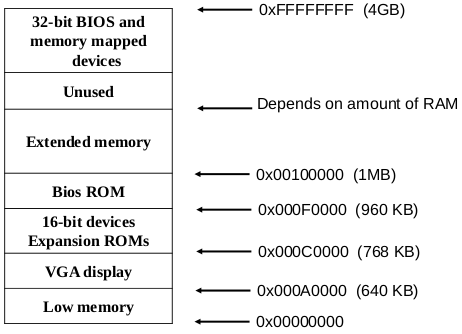
\includegraphics[scale=0.4]{images/device_management/booting_memory.png}
\caption{UNIX Memory Organization}
\end{figure}

The first PCs, which were based on the 16-bit Intel 8088 processor, were only capable of addressing 1MB of physical memory. The physical address space of an eary PC would therefore start at 0x00000000 but end at 0x000FFFFF instead of 0xFFFFFFFF.
\begin{itemize}
\item The 640KB area marked ``Low Memory'' was the \textit{only} random-access memory (RAM) that an early PC could use;
\item The 348KB area from 0x000A0000 through 0x000FFFFF was reserved by the hardware for special uses such as video display buffers and firmware held in nonvolatile memory;
\item The most important part of this reserved area is the Basic Input/Output System (BIOS), which occupies the 64KB region from 0x000F0000 through 0x000FFFFF.
\end{itemize}

Intel 80286 and 80836 processors supported 16MB and 4GB physical address spaces respectively, but the PC architects preserved the original layout for the low 1MB of physical address space for backward compatibility with existing software. Modern PCs therefore have a ``hole'' in physical memory from 0x000A0000 to 0x00100000, dividing RAM into ``low'' or \emph{conventional memory} (the first 640KB) and \emph{extended memory} (everything else).
More BIOS is located at the high end of the 32-bit address range for use by 32-bit PCI devices.

\subsection{The BIOS}
The BIOS is responsible for performing \emph{Power-On-Self-Test} and basic system initialization such as activating the video card and checking the amount of memory installed. After performing this initialization, the BIOS loads the operating system from some appropriate location such as floppy disk, hard disk, CD-ROM, or the network, and passes control of the machine to the operating system.

486 and later processors start executing at physical address 0xFFFFFFF0, which is at the very top of memory space, in an area reserved for the ROM BIOS. The first instruction is \texttt{jmp far F000:E05B} which jumps to the normal BIOS, located in the 64KB region from 0xF0000 to 0xFFFFF mentioned above. The CPU starts in \emph{real mode}, so the \texttt{jmp far} instruction is a real mode jump that restores us to low memory. In real mode, the segmented address \texttt{segment:address} translates to the physical address \texttt{segment*16 + offset}. Thus, F000:E05B translates to 0x000FE05B.

In real mode, nether Global Descriptor Table (GDT) nor Local Descriptor Table (LDT) (which, in protected mode, contain global and local segment descriptions respectively) are needed by the CPU. The code that initializes these data structures must run in real mode. When the BIOS run, it initializes the PCI bus and all the important devices it knows about (in particular VGA display), then it searches for a bootable device such as a floppy disk, hard drive or CD-ROM and when it find it, it reads the boot loader from the disk and transfers control to it.

\subsection{The Boot Loader}
The \emph{Boot Loader} is the program run by the BIOS to load the image of a kernel into RAM. Floppy and hard disks are by historical convention divided up into 512 byte regions called \emph{sectors}. If the disk is bootable, the first sector is called the \emph{boot sector}, since this is where the Boot Loader code resides. When the BIOS find a bootable floppy or hard disk, it loads the 512-byte boot sector into lowe memory, at physical address 0x7C00 through 0x7DFF and then it uses a \texttt{jmp} instruction to set the \texttt{CS:IP} to 0000:7C00, passing control to the Boot Loader.

Boot Loader important files are:
\begin{itemize}
\item \texttt{boot.s} - First, the boot loader switches the processor from real mode to 32-bit protected mode, because  it is only in this mode that software can access all the memory above 1MB in the processor's physical address space;
\item \texttt{main.c} - Second, the boot loader reads the kernel from the hard disk by directly accessing the IDE disk device registers via the x86's special I/O instructions;
\item \texttt{boot.asm} - This file is a disassembly of the boot loader. It easy to see exactly where in the physical memory all of the boot loader's code resides.
\end{itemize}

The boot loader's link and load addresses match perfectly. There is a rather large disparity between the kernel's link and load addresses. Operating system kernels often like to be linked and run at very high virtual address, such as 0xF0100000, in order to leave the lower part of the processor's virtual address space for user programs to use. Actually, it is not possible to load the kernel at \textit{physical address} 0xF0100000, then it is needed to use the processor's memory management hardware to map virtual address 0xF0100000 - link address where the kernel code \emph{expects} to run - to physical address 0x00100000 - where the boot loader \textit{actually} loaded the kernel. The kernel's virtual memory address is high enough to leave plenty of address space for user processes, it will be loaded in physical memory at the 1MB point in the PC's RAM, just above the BIOS ROM.

\section{I/O subsystem}
\begin{figure}[hbtp]
\centering
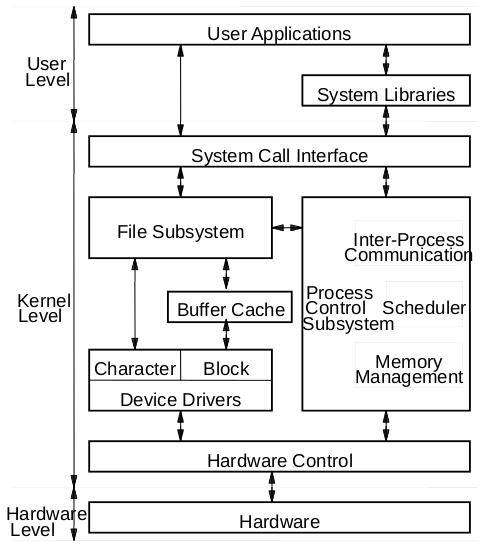
\includegraphics[scale=0.4]{images/device_management/unix_io_subsystem.png}
\caption{UNIX I/O subsystem}
\end{figure}
User application access to a wide variety of different devices is accomplished through layering and through encapsulating all the device-specific code into device drivers, while application layers are presented with a common interface for all (or at least large general categories of) devices. Most devices can be characterized as either block I/O, character I/O, memory mapped file access or network sockets. A few devices are special, such as time-of-day clock and the system timer. Most operating systems also have an escape, or back door, which allows applications to sens command directly to device drivers if needed. In UNIX this is \texttt{ioctl()} system call. \texttt{ioctl()} takes three arguments: the file descriptor for the device driver being accessed, an integer indicating the desired function to be performed and an address used for communicating or transferring additional information.

\subsection{Block and Character Devices}
Block devices are accessed one block at a time, and are indicated by a \texttt{b} as the first character in a long listing on UNIX systems. Operations supported include \texttt{read}, \texttt{write} and \texttt{seek}. Accessing blocks on a hard drive directly, without going through the filesystem structure, is called \emph{raw I/O} and can speed up certain operation by bypassing the buffering and locking normally introduced by the OS, i.e.\@ it becomes the application's responsibility to manage those issues. A new alternative is \emph{direct I/O}, which uses the normal filesystem access, but which disables buffering and locking operations. Memory mapped file I/O can be layered on top of block-device drivers. Rather than reading the entire file, it is mapped to a range of memory addresses and then paged into memory as needed using the virtual memory mechanism. Access to the file is then accomplished through normal memory access, i.e.\@ pointers, rather than through \texttt{read} and \texttt{write} system calls. This approach is commonly used for executable program code.

\begin{figure}[hbtp]
\centering
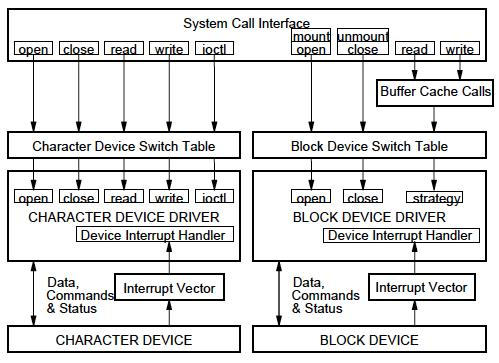
\includegraphics[scale=0.4]{images/device_management/unix_sw_interface.jpg}
\caption{UNIX software interface}
\end{figure}

Character devices are accessed one byte at a time, and are indicated by a \texttt{c} in UNIX systems. Supported operations include \texttt{get} and \texttt{put}, with more advanced functionality such as reading an entire line supported by higher-level library routines.

\subsection{Filesystem data structures}
In the original UNIX filesystem, the physical disks is divided into logical disks called \emph{partitions}. Each partition is a standalone filesystem. Each device in the system is characterized by its own major device number and each partition has an associated minor device number which the device drivers uses to access the raw filesystem. The major/minor device number combination is used as an handle into device switch table. In particular, the major number acts as an index, and the minor number is passed as an argument to the driver routines so that they can recognize the specific instance of a device.

Each filesystem contains:
\begin{itemize}
\item a \emph{boot block} located in the first few sectors of a filesystem. The boot block contains the initial bootstrap program used to load the operating system. Typically, the first sector contains a bootstrap program that reads in a larger bootstrap program from the next few sector, and so forth;
\item a \emph{superblock} describes the state of the filesystem: the total size of the partition, the block size, pointers to a list of free blocks, the i-node number of the root directory, magic number, etc.;
\item a linear \emph{array of i-nodes}. There is a one to one mapping of files to i-nodes and viceversa. An i-node is identified by its \emph{i-node number}, which  contains the information needed to find the i-node itself on the disk. Thus, while users think of files in terms of file names, UNIX thinks of files in terms of i-nodes.
\item a \emph{data blocks} containing the actual content of files.
\end{itemize}

System calls like \texttt{mkfs} can be used to create (format) the filesystem (partition). Indeed, it creates the superblock, the i-node list, the list of free blocks and the root node for the new filesystem. Other system calls like \texttt{fsck}, instead, are used to check and repair the filesystem.

Therefore, it is simple to understand that there is a similarity between normal files and device in a UNIX filesystem: both are characterized by an i-node.

\begin{figure}[hbtp]
\centering
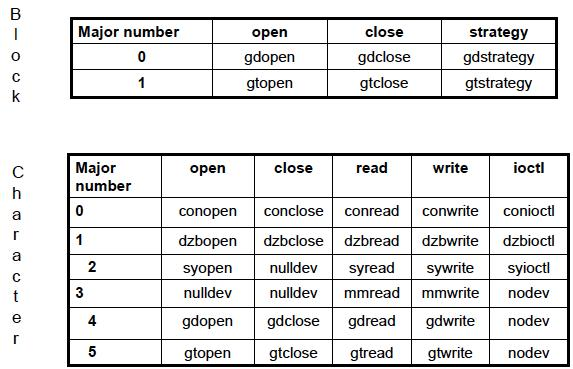
\includegraphics[scale=0.4]{images/device_management/unix_switch_tables.jpg}
\caption{UNIX switch tables}
\end{figure}

\paragraph{Open system call for I/O devices}
\begin{enumerate}
\item Convert pathname into i-node;
\item Increase the i-node reference counter;
\item Allocate an element into user file table and system file table;
\item Get major and minor number from i-node;
\item Save content using \texttt{setjmp}\footnote{Saves the current context (environment) in the stack. Used to backtrack in case of errors, instead of a chain of \texttt{return} statements} to resolve a possible \texttt{longjmp} executed by the driver;
\item If device is a block device:
\begin{enumerate}
\item Use major number as an index into block device switching table;
\item Call open procedure of the driver associated to the index above passing minor number and mode;
\end{enumerate}
\item Otherwise:
\begin{enumerate}
\item Use major number as an index into character device switching table;
\item Call open procedure of the driver associated to the index above passing minor number and mode;
\end{enumerate}
\item If open fails, decrease counters in file and i-node tables.
\end{enumerate}

\subsection{Terminal driver}
A multiplicity of I/O devices are regarded as ``terminals'' in Unix systems. A terminal is a character-oriented device, comprising streams of characters received from and sent to the device. Although characters streams are structured, incorporating control characters, escape codes and special characters, the I/O protocol is not structured as would be the I/O protocol of smart terminals. Terminals provide job control facilities: interactively, the user and the terminal can send control characters that suspend the current running job, reverting to the interactive job control shell that spawned the job and can run commands which place jobs in background or which switch a background job into foreground, without suspending it if necessary.

In UNIX, a terminal device comprises the underlying \emph{device driver}, responsible for the physical control of the device hardaware via the I/O instructions and handling device interrupt requests, and the \emph{line discipline}, as shown in figure~\ref{unix_line_discipline}. A line discipline is independent from the actual device hardware, and the same line discipline can be used for a terminal concentrator device responsible for multiple controlling terminals as for a pseudoterminal. Line disciplines can be setup by functions or system calls. They are the same across all terminal devices and independent from the actual hardware, dealing as they do in the simple abstractions provided by device drivers: transmit and receive a character and set different hardware states. Each terminal device can be switched among multiple line disciplines.

\begin{figure}[hbtp]
\centering
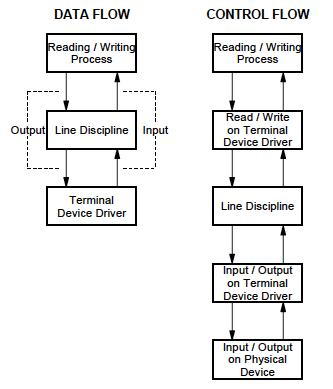
\includegraphics[scale=0.6]{images/device_management/unix_line_discipline.jpg}
\caption{UNIX line discipline}
\label{unix_line_discipline}
\end{figure}

Every line discipline may operate in two modes:
\begin{itemize}
\item \textbf{Raw mode}: the line discipline transfers data between a terminal and a process without any conversion. The \texttt{enter} character has no specific meaning in this mode. The behavior of the raw mode can be set using the \texttt{ioctl} system call;
\item \textbf{Canonical mode}: characters are got into kernel buffer and passed to the process only when \texttt{ENTER} is pressed. The user input is converted for the receiving process and the process output is converted for the user. It manages \texttt{backspace}, formatting characters such as \texttt{tab} and \texttt{enter} and special characters such as \texttt{Ctrl-C}, \texttt{Del} and \texttt{Ctrl-D}.
\end{itemize}

The POSIX standard replaces the \texttt{ioctl} system call entirely, with a set of library functions with standardized names and parameters. The POSIX \texttt{termio} data structure is the data structure used by all of the terminal library calls.
\begin{verbatim}
struct termios {
  tcflag_t c_iflag;  // Input mdoes
  tcflag_t c_oflag;  // Output modes
  tcflag_t c_cflag;  // Control modes
  tcflag_t c_lflag;  // Local modes
  cc_t c_cc[NCCS];   // Control characters
};
\end{verbatim}
Each process in the system has either a single controlling terminal, or no controlling terminal at all. A process inherits its controlling terminal from its parent, and the only operations upon a process are acquiring a controlling terminal, by a process that has no controlling terminal, and relinquishing it, by a process that has a controlling terminal. The standard defines the \texttt{O\_NOCTTY} flag for the \texttt{open} system call. A process with no controlling terminal opens a terminal device file that is not already the controlling terminal for some other process, without specifying the \texttt{O\_NOCTTY} flag.

\subsubsection{\texttt{getty}}
\texttt{getty} (get teletype) is a typical UNIX system program used to manage physical and virtual terminals. When it detects a connection, it prompts for a username password an runs the ``login'' program to authenticate the user.

At the login phase, the \texttt{init} process reads \texttt{/etc/inittab} and executes a \texttt{getty} process for each known terminal that has been switched on. Then, \texttt{getty} calls the system call \texttt{open} related to the terminal, which makes the process wait for the hardware connection has been established. The \texttt{getty} program, through system call \emph{exec}, becomes the \texttt{login} process, which runs, exploiting system call \texttt{exec}, the user selected shell reading the last field of the username record in file \texttt{/etc/passwd}.

\subsection{Buffer cache}
In order to speedup the read request from a device, it is possible to use buffers and/or caches which allow a faster communication to take place

When the kernel is asked to serve a \textbf{read} request from disk, it tries to read the data from the \emph{buffer cache}. If the data are in the cache, the data are returned to the user process without any disk access, otherwise the kernel reads a block of data from disk and stores it in the buffer cache, trying to keep it in memory as long as possible, for a possible future usage.

When the kernel is asked to serve \textbf{write} request to disk, it puts the data in the buffer cache. In this way, data stay in memory for possible read operations and any change of the data is performed in memory rather than on disk.

The buffer cache management tries to minimize the number of disk accesses by \emph{reading ahead} the data that have high probability\footnote{According to the space and temporal locality principle} to be referenced in the near future and by delaying as much as possible the transfer of the content of the buffer cache to disk (\emph{delayed write}).

\subsection*{Read system call}
\begin{verbatim}
procedure read
input:  user file descriptor
        user buffer address
        number of bytes to read
output: number of bytes copied in the user buffer
{
  while(! complete number of bytes to read) {
    convert offset to byte in a block (using bmap);
    compute the offset within a block
      and the number of byte to read;
    if(number of byte to read == 0)
      break;  /* tries to read beyond the end of file */
    read a block (using bread or breada);
    copy data from kernel buffer to user space;
    release buffer (using brelse);
    
    return number of bytes; 
}
\end{verbatim}

\subsection*{Block read: \texttt{bread}}
\begin{verbatim}
procedure bread
input:  filesystem block number (blockno)
output: buffer containing requested block
{
  buffer = getblock(block blockno);
  if(data in buffer are valid)
    return buffer;
  start disk I/O read for block blockno into buffer;
  sleep(event: disk I/O read completed);
  return buffer;
}
\end{verbatim}

\subsection*{Acquiring a block: \texttt{getblk}}
\begin{verbatim}
procedure getblk
input:  device number
output: locked buffer to be used for storing the block
{
  while(buffer not found) {
    if(block is present in its hash queue) {
      /* Case 5 */
      if(buffer is locked) {
        sleep(event: buffer unlocked);
        continue;
      }
      /* Case 1 */
      mark buffer 'locked';
      remove buffer from free list;
      return buffer;
    } else {
      if(free list is empty) {
        /* Case 4 */
        sleep(event: freed buffer);
        continue;
      }
      remove buffer from free list;
      if(buffer marked 'delayed write') {
        /* Case 3 */
        asynchronous disk write of buffer;
        continue;
      }
      /* Case 2 */
      remove buffer from old hash queue;
      put buffer into new hash queue;
      return buffer;
    }
  }
}
\end{verbatim}

\subsection*{Block release: \texttt{brelse}}
\begin{verbatim}
procedure brelse
input:  locked buffer
output: none
{
  wake up all processes waiting for any free buffer;
  wake up all processes waiting for this buffer;
  disable interrupts;
  if(buffer contents are valid and buffer not old) {
    put buffer in free list queue;
  else
    put buffer in free list head;
  enable interrupts;
  mark buffer unlocked;
}
\end{verbatim}

\subsection*{Block write: \texttt{bwrite}}
\begin{verbatim}
procedure bwrite
input:  buffer to write
output: none
{
  start disk I/O write of buffer;
  if(synchronous I/O) {
    sleep(event: disk I/O write completed);
    brelse(buffer);
  } else if(buffer is marked delayed write)
    mark buffer 'old';
}
\end{verbatim}

\subsection*{Block read ahead: \texttt{breada}}
\begin{verbatim}
procedure breada
input:  filesystem block number for immediate read (blkno1)
        filesystem block number for asynchronous read (blockno2)
output: buffer containing data from immediate read (buffer1)
{
  if(buffer with blkno1 not present in buffer cache) {
    buffer1 = getblk(block blkno1);
    if(data in buffer1 are not valid)
      start disk I/O read for blockno1 into buffer1;
  }
  if(buffer with blkno2 not present in buffer cache) {
    buffer2 = getblk(block blkno2);
    if(data in buffer2 are valid)
      brelse(buffer2);
    else
      start disk I/O read for block blkno2 into buffer2;
  }
  if(buffer with blkno1 present in buffer cache) {
    buffer1 = bread(blkno1);
    return buffer1;
  }
  sleep(event: blkno1 disk I/O read completed);
  return buffer1;
}
\end{verbatim}